\section{Simulation Study}

\begin{frame}
    \frametitle{Simulation Study: Linear DGP}
    The linear DGP generates the data tuples \( (y, x_{1}, x_{2}, x_{3}) \) as follows:

    \begin{equation}\label{eq:linear_dgp}
        y = \beta_{0} + \beta_{1} x_{1} + \beta_{2} x_{2} + \beta_{3} x_{3} + \epsilon,
    \end{equation}
    
    whereas \( (\beta_{0}, \beta_{1}, \beta_{2}, \beta_{3}) = (0.3, 5, 10, 15) \),
    \( x_{1}, x_{2}, x_{3} \sim \mathcal{N}(0,\,3) \), and \( \epsilon \sim \mathcal{N}(0,\,1) \).
\end{frame}

\begin{frame}
	\frametitle{Decision Tree: Linear DGP Results}
	\begin{center}		
		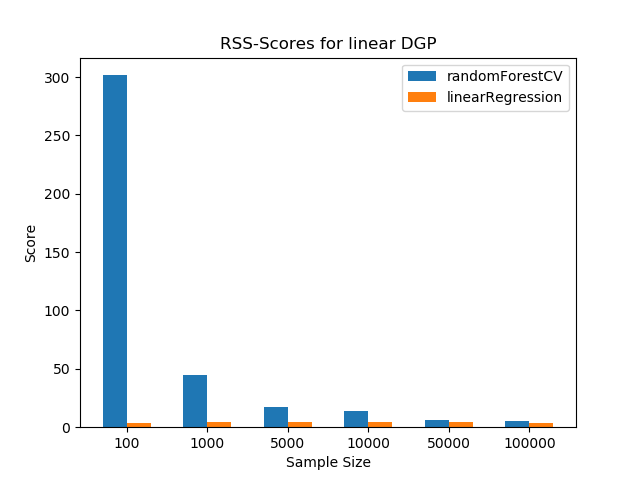
\includegraphics[height=0.7\textheight]{images/forest_vs_ols_linearDGP.png}
	\end{center}
\end{frame}


\begin{frame}
    \frametitle{Simulation Study: Non-Linear DGP}
    The non-linear DGP generates the data tuples \( (y, x_{1}, x_{2}) \) as follows:

    \begin{equation}\label{eq:non_linear_dgp}
        y = \beta_{0} + \beta_{1} \mathds{1}(x_{1} \geq 0, x_{2} \geq 0) + \beta_{2} \mathds{1}(x_{1} \geq 0, x_{2} < 0) + \beta_{3} \mathds{1}(x_{1} < 0) + \epsilon,
    \end{equation}
    
    whereas \( (\beta_{0}, \beta_{1}, \beta_{2}, \beta_{3}) \), \( x_{1}, x_{2} \) and \(  \epsilon \)
    are the same as in the previous DGP.
\end{frame}

\begin{frame}
	\frametitle{Simulation Study: Non-Linear DGP Results}
	\begin{center}		
		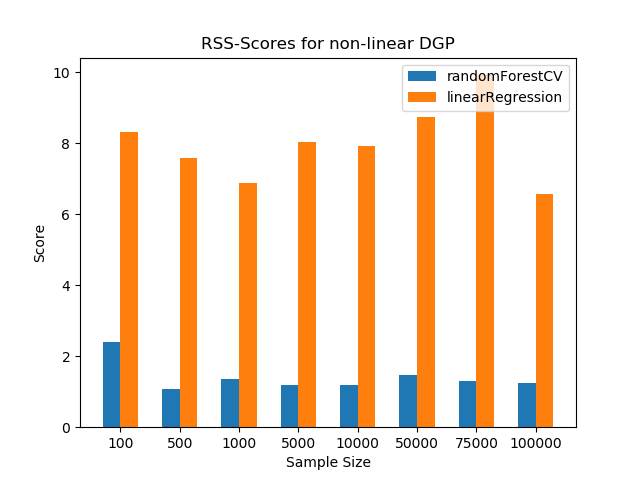
\includegraphics[height=0.7\textheight]{images/forest_vs_ols_nonlinearDGP.png}
	\end{center}
\end{frame}